\documentclass{beamer}
\usepackage[utf8]{inputenc}
\usepackage[brazil]{babel}
\usepackage{amsmath}
\usepackage{caption}
\usepackage{array}
\usepackage{subcaption}

\title{Determinantes macroeconômicos do spread bancário ex-ante brasileiro: uma abordagem econométrica (2011-2019)}
\author{Phelipe Teles}
\date{2019}
\institute{Universidade Federal Rural do Rio de Janeiro}

\usepackage{graphicx}
\graphicspath{{../graficos/}}

\begin{document}

\frame{\titlepage}

\begin{frame}
    \frametitle{Spread bancário na América Latina}
    \centering
    \begin{figure}
        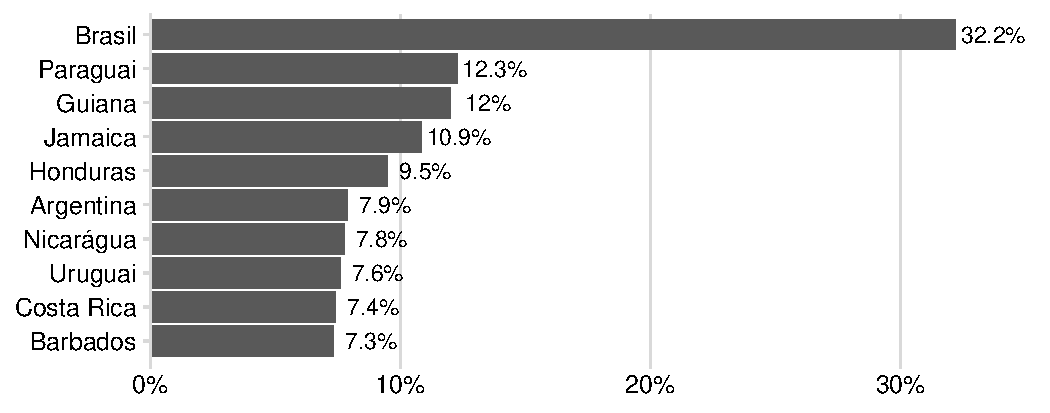
\includegraphics[scale=.6]{spread_AL.pdf}
    \end{figure}
\end{frame}

\begin{frame}
    \frametitle{Spread bancário (2011-2019)}
    \centering
    \begin{figure}[htbp]
        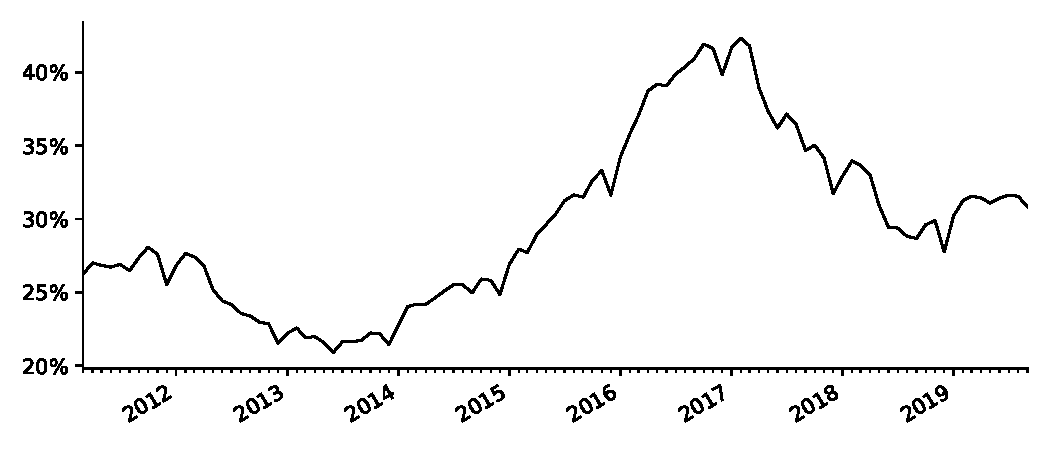
\includegraphics[width=\textwidth, scale=.6]{spread.pdf}
    \end{figure}
\end{frame}

\begin{frame}
    \frametitle{Literatura teórica I}
    \begin{enumerate}
        \item O banco como firma - Klein (1971)
            \begin{enumerate}
                \item Banco como agente neutro ao risco, maximizador do lucro esperado.
                \item Spread como poder de mercado (mark-up).
            \end{enumerate}
        \item Principais Determinantes
            \begin{enumerate}
                \item Taxa de juros.
                \item Market-share.
            \end{enumerate}
    \end{enumerate}

\end{frame}

\begin{frame}
    \frametitle{Literatura teórica II}
    \begin{enumerate}
        \item O banco como intermediador financeiro (1981)
            \begin{enumerate}
                \item Banco como agente avesso ao risco.
                \item Spread como proteção ao risco da taxa de juros e da inadimplência.
                \item Metodologia de dois passos para a estimação.
            \end{enumerate}
        \item Principais Determinantes
            \begin{enumerate}
                \item Taxa de juros e sua volatilidade.
                \item Estrutura competitiva do mercado.
                \item Aversão ao risco.
                \item Inadimplência
                \item Escala de operação.
            \end{enumerate}
    \end{enumerate}

\end{frame}

\begin{frame}
\renewcommand{\arraystretch}{2.0}
    \frametitle{Tabela-resumo da revisão da literatura empírica}
    \begin{table}[ht]
        \resizebox{8cm}{!}{
            \begin{tabular}{|l|l|p{5cm}|}
            \hline
            Estudo & Período & Resultados \\
            \hline
            Afanasieff, Lhacer e Nakane (2002) & fev/1997 -- nov/2000 & IGP (-), Crescimento do produto industrial (-), Selic (+), Volatilidade Selic (-) \\
            \hline
            Koyama e Nakane (2002) & ago/1994 -- set/2001 & Selic(+), \textit{Spread over treasury} (+), Impostos indiretos (+), Reservas compulsórias (0), C. administrativo (+) \\
            \hline
            Bignotto e Rodrigues (2006) & mar/2001 -- mar/2004 & IPCA (-), Selic (+), Despesas tributárias (0), C. Administrativos (+), Risco de juros (+), Risco de crédito (+), Parcela de mercado (-), Liquidez (+), Receita serviços (+), Compulsório (+), Ativo total (+)  \\
            \hline
            Oreiro et. al (2006) & jan/1995 -- dez/2003 & IPCA(0), Produto Industrial (+), Selic (+), Volatilidade Selic (+) \\
            \hline
            Chaim (2013) & jan/2004 -- dez/2012 & Selic (+), \textit{Spread over treasury} (+), Taxa de câmbio (+), Inflação (+), Produção Industrial (+) \\
            \hline
        \end{tabular}}
    \end{table}
\end{frame}

\begin{frame}
    \frametitle{Séries incluídas no modelo}
    \begin{figure}[htbp]
        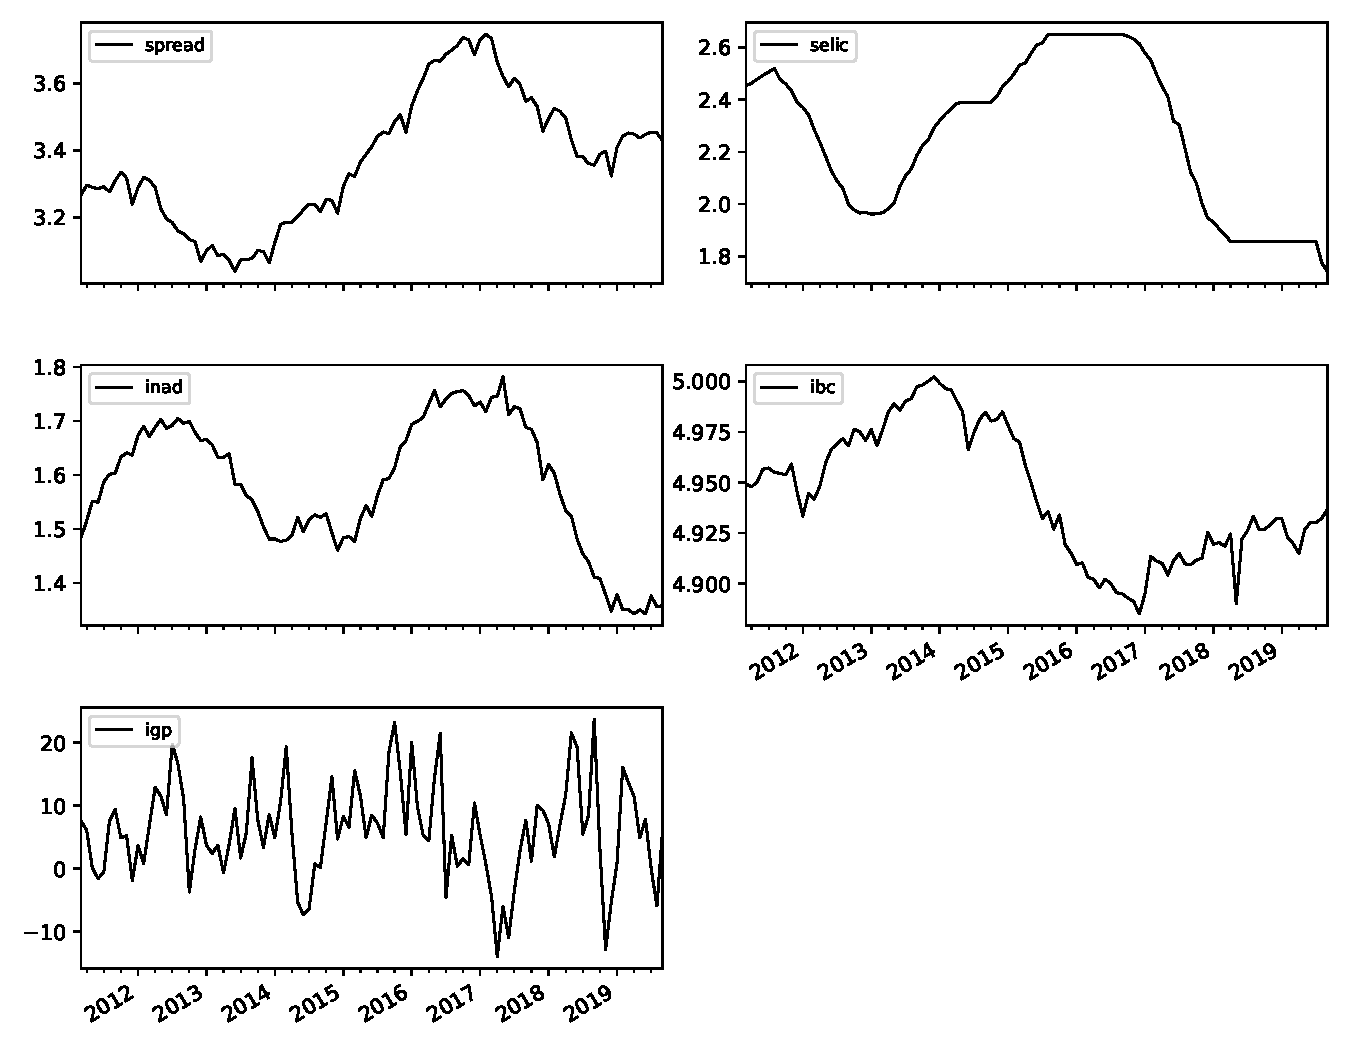
\includegraphics[width=\textwidth, height=.8\textheight, scale=1]{series_modelo.pdf}
    \end{figure}
\end{frame}


\begin{frame}
    \frametitle{Estatísticas descritivas e sinais esperados das variáveis}
    \centering
    \renewcommand{\arraystretch}{1.5}
    \begin{table}[h]
        \resizebox{10cm}{!}{
            \begin{tabular}{|l|c|c|c|c|c|}
                \hline
                Variável              & Média & Desvio Padrão & Mín. & Máx. & Sinal esperado \\
                \hline
                Spread                & 29,33      & 6,51    & 20,89     & 42,34  &  \\
                Selic                 & 10,96      & 2,37    & 7,00      & 14,15  & + \\
                Inadimplência         & 5,09       & 0,47    & 4,31      & 5,94   & + \\
                IGP-DI                & 5,74       & 7,33    & $-$13,93  & 23,26  & + \\
                Atividade Econômica   & $-$2,28    & 4,86    & $-$13,39  & 9,70   & +/- \\
                IHH                   & 1.566,30   & 133,69  & 1.357     & 1.751  & + \\
                \hline
            \end{tabular}}
    \end{table}
\end{frame}

\newcolumntype{C}[1]{>{\centering\arraybackslash}p{#1}}

\begin{frame}
    \frametitle{Testes de raiz unitária I}
    \framesubtitle{Augmented Dickey Fuller}
    \renewcommand{\arraystretch}{1.2}
    \begin{table}[ht]
        \resizebox{10cm}{!}{
        \begin{tabular}{|l|c|c|c|c|}
            \hline
            & & \multicolumn{1}{C{3cm}}{Sem drift e sem tendência}  & \multicolumn{1}{C{3cm}}{Com drift} & \multicolumn{1}{C{3cm}|}{Com tendência} \\
            \hline
            Variável & Defasagem & \multicolumn{3}{c|}{P-valor} \\
            \hline
            spread*      &         12 &     0.67 &     0.12 &     0.00 \\
            selic        &          4 &     0.23 &     0.61 &     0.79 \\
            ibc          &          0 &     0.59 &     0.68 &     0.75 \\
            inad         &          4 &     0.37 &     0.17 &     0.39 \\
            igp*         &          0 &     0.00 &     0.00 &     0.00 \\
            \hline
        \end{tabular}}
    \caption*{$ \text{H}_0 $: raiz unitária. $ \text{H}_a $: estacionária.}
    \end{table}
\end{frame}

\begin{frame}
    \frametitle{Testes de raiz unitária II}
    \framesubtitle{Philips Perron}
    \renewcommand{\arraystretch}{1.2}
    \begin{table}[ht]
        \resizebox{10cm}{!}{
        \begin{tabular}{|l|c|c|c|c|}
            \hline
            & & \multicolumn{1}{C{3cm}}{Sem drift e sem tendência}  & \multicolumn{1}{C{3cm}}{Com drift} & \multicolumn{1}{C{3cm}|}{Com tendência} \\
            \hline
            Variável & Defasagem & \multicolumn{3}{c|}{P-valor} \\
            \hline
            spread     &         13 &     0.76 &     0.61 &     0.79 \\
            selic      &         13 &     0.31 &     0.76 &     0.90 \\
            ibc        &         13 &     0.60 &     0.61 &     0.65 \\
            inad       &         13 &     0.54 &     0.57 &     0.72 \\
            igp*        &         13 &     0.00 &     0.00 &     0.00 \\
            \hline
        \end{tabular}}
    \caption*{$ \text{H}_0 $: raiz unitária. $ \text{H}_a $: estacionária.}
    \end{table}
\end{frame}

\begin{frame}
    \frametitle{Testes de raiz unitária III}
    \framesubtitle{KPSS}
    \renewcommand{\arraystretch}{1.2}
    \begin{table}[ht]
        \resizebox{10cm}{!}{
            \begin{tabular}{|l|c|c|c|c|}
                \hline
                & \multicolumn{2}{C{5cm}}{$ \text{H}_0 $: constante-estacionária} & \multicolumn{2}{C{5cm}|}{$ \text{H}_0 $: tendência-estacionária} \\
                \hline
                Variável & Defasagem & P-valor & Defasagem & P-valor \\
                \hline
                spread     &          6 &     0.01 &          5 &     0.01 \\
                selic*      &          6 &     0.09 &          6 &     0.01 \\
                ibc        &          5 &     0.01 &          5 &     0.01 \\
                inad*       &          5 &     0.10 &          5 &     0.02 \\
                igp*        &          4 &     0.10 &          4 &     0.10 \\
                \hline
            \end{tabular}
        }
        \caption*{$ \text{H}_0 $: estacionariedade. $ \text{H}_a $: raiz unitária.}
    \end{table}
\end{frame}

\begin{frame}
    \frametitle{Teste de Co-integração uni-equacional}
    \framesubtitle{Teste de Engle-Granger}
    \begin{table}[hbt]
        \resizebox{10cm}{!}{
        \begin{tabular}{|cccccc|}
            \hline
            Tendência & Engle-Granger & P-valor & 1\% & 5\% & 10\% \\
            \hline
            Sim & -5.16 & 0.01 & -5.2 & -4.57 & -4.26 \\
            Não & -4.84 & 0.01 & -4.83 & -4.21 & -3.89 \\
            \hline
        \end{tabular}}
    \end{table}
\end{frame}

\begin{frame}
    \frametitle{Equação do vetor co-integrante}
    \begin{align*}
        \resizebox{\hsize}{!}{
            spread_t - \beta_0 - \beta_1 selic_t - \beta_2 inad_t -\beta_2 ibc_t = u_t
        }
    \end{align*}
\end{frame}



\begin{frame}
    \frametitle{Estimação relação de co-integração uni-equacional}
    \begin{table}[!hbt]
        \centering
        \renewcommand{\arraystretch}{1.2}
        \resizebox{6cm}{!}{
        \begin{tabular}{@{\extracolsep{20pt}}lcc}
            \hline
            \hline
            & \multicolumn{1}{c}{Variável dependente:} \\
            \cline{2-2}
            & spread \\
            \hline
            Intercept         & 30.2636***       \\
            & (1.0014)         \\
            selic             & 0.1619***        \\
            & (0.0238)         \\
            inad              & -0.0839          \\
            & (0.0596)         \\
            ibc               & -5.4874***       \\
            & (0.1967)         \\
            \hline
            Observações       & 102.0000         \\
            $ R^2 $           & 0.9056           \\
            $ R^2 $ Ajustado  & 0.9027           \\
            Estatística F     & 313.346 (0.000)  \\
            Jarque-Bera       & 1.806 (0.405)    \\
            Dickey-Fuller     & -4.156 (0.001)   \\
            Durbin-Watson     & 0.706            \\
            \hline
            \hline
        \end{tabular}}
    \end{table}
\end{frame}

\begin{frame}
    \frametitle{Modelo de correção de erros}
    \begin{align*}
        \resizebox{\hsize}{!}{
            \Delta \textit{spread} = \alpha (\textit{spread} - \hat{\beta_0} - \hat{\beta_1} \textit{selic} -\hat{\beta_2} \textit{inad} + \hat{\beta_3} \textit{igp)}\ +\ \alpha_1 \Delta \textit{selic}\ +\ \alpha_2 \Delta \textit{inad}\ +\ \alpha_3 \Delta \textit{igp} + u_t
        }
    \end{align*}
\end{frame}


\begin{frame}
    \frametitle{Estimação do modelo de correção de erros}
    \begin{table}[!hbt]
        \centering
        \renewcommand{\arraystretch}{1.2}
        \resizebox{6cm}{!}{
            \begin{tabular}{@{\extracolsep{20pt}}lcc}
                \hline
                \hline
                & \multicolumn{1}{c}{Variável dependente:} \\
                \cline{2-2}
                & spread \\
                \hline
                equilibrio        & -0.1009*        \\
                & (0.0547)        \\
                selic             & 0.2186**        \\
                & (0.0936)        \\
                inad              & 0.5216***       \\
                & (0.1317)        \\
                ibc               & -0.4502         \\
                & (0.4184)        \\
                \hline
                Observações       & 101.0000        \\
                $ R^2 $           & 0.2862          \\
                $ R^2 $ Ajustado  & 0.2567          \\
                Estatística F     & 9.722 (0.000)   \\
                Jarque-Bera       & 3.023 (0.221)   \\
                Dickey-Fuller     & -8.347 (0.000)  \\
                Durbin-Watson     & 1.781           \\
                \hline
                \hline
            \end{tabular}}
    \end{table}
\end{frame}


\begin{frame}
    \frametitle{Modelo vetorial de correção de erros}
    \begin{equation*}
    \resizebox{.9\hsize}{!}{
        \Delta y_t = \alpha \beta^{'} y_{t-1}+ \Gamma_1 \Delta y_{t-1} + \cdots + \Gamma_{p} \Delta y_{t-1} + CD_t + u_t \label{vecm_spread}
    }
    \end{equation*}
\end{frame}

\begin{frame}
    \frametitle{Autocorrelação residual}
    \framesubtitle{Teste de Portmeanteau}
    \begin{table}[!hbt]
        \begin{tabular}{|cccc|}
            \hline
            Estatística de teste & Valor crítico & P-valor & Graus de liberdade  \\
            \hline
            170.4          &          186.1          &      0.203       &     156      \\
            \hline
        \end{tabular}
        \caption*{$ \text{H}_0 $: Resíduos são correlacionados até lag 12. \newline $ \text{H}_a $: Resíduos não correlacionados}
    \end{table}
\end{frame}


\begin{frame}
    \frametitle{Normalidade dos resíduos}
    \framesubtitle{Teste de Jarque-Beta}
    \begin{table}[!hbt]
        \begin{tabular}{|cccc|}
            \hline
            Estatística de teste & Valor crítico & P-valor & Graus de liberdade  \\
            \hline
            117.2          &          15.51          &      0.000       &      8       \\
            \hline
        \end{tabular}
        \caption*{$ \text{H}_0 $: Resíduos não são normalmente distribuídos. \newline $ \text{H}_a $: Resíduos são normalmente distribuídos.}
    \end{table}
\end{frame}

\begin{frame}
    \frametitle{Teste de co-integração multi-equacional}
    \framesubtitle{Teste de Johansen (traço)}
    \begin{table}[!hbt]
        \begin{tabular}{|cccc|}
            \hline
            $ r_0 $ & $ r_1 $ & Estatística de teste & Valor Crítico \\
            \hline
            0 &             1 &                   33.52 &                   30.82  \\
            1 &             2 &                   16.57 &                   24.25  \\
            \hline
        \end{tabular}
        \caption*{$ \text{H}_0 $: $ r =  r_0 $. $ \text{H}_a $: $ r_0 = r_0 + 1 $}
    \end{table}
\end{frame}

\begin{frame}
    \frametitle{Teste de co-integração multi-equacional}
    \framesubtitle{Teste de Johansen (máximo autovalor)}
    \begin{table}[!hbt]
        \begin{tabular}{|cccc|}
            \hline
            $ r_0 $ & $ r_1 $ & Estatística de teste & Valor Crítico \\
            \hline
            0 &             4 &                   60.57 &                   55.25  \\
            1 &             4 &                   27.05 &                   35.01  \\
            \hline
        \end{tabular}
        \caption*{$ \text{H}_0 $: $ r =  r_0 $. $ \text{H}_a $: $ r_0 < r < 4 $}
    \end{table}
\end{frame}

\begin{frame}
    \frametitle{Estimação do modelo vetorial de correção de erros}
    \framesubtitle{Coeficientes do vetor co-integrante}
    \renewcommand{\arraystretch}{1.2}
    \begin{table}[!hbt]
        \resizebox{10cm}{!}{
            \begin{tabular}{|ll|cccccc|}
                \hline
                & & Coeficiente & Desvio Padrão    & Z          & P$>|$z$|$           & [0.025          & 0.975]  \\
                \hline
                spread    & $ \hat{\alpha_1}  $        &      -0.0764         &        0.031     &    -2.463  &         0.014        &       -0.137    &       -0.016     \\
                selic     & $ \hat{\alpha_2}  $        &      -0.0302         &        0.035     &    -0.863  &         0.388        &       -0.099    &        0.038     \\
                ibc       & $ \hat{\alpha_3}  $        &      -0.0362         &        0.014     &    -2.518  &         0.012        &       -0.064    &       -0.008     \\
                inad      & $ \hat{\alpha_4}  $        &      -0.1603         &        0.026     &    -6.182  &         0.000        &       -0.211    &       -0.109     \\
                spread   & $ \hat{\beta_1}  $         &       1.0000         &            0     &         0  &         0.000        &        1.000    &        1.000     \\
                selic    & $ \hat{\beta_2}  $         &      -0.4674         &        0.040     &   -11.783  &         0.000        &       -0.545    &       -0.390     \\
                ibc      & $ \hat{\beta_3}  $         &       5.2031         &        0.228     &    22.773  &         0.000        &        4.755    &        5.651     \\
                inad     & $ \hat{\beta_4}  $         &       0.5153         &        0.083     &     6.185  &         0.000        &        0.352    &        0.679     \\
                \hline
            \end{tabular}
        }
    \end{table}
\end{frame}

\begin{frame}
    \frametitle{Estimação do modelo vetorial de correção de erros}
    \framesubtitle{Funções de Impulso-resposta}
    \begin{figure}[!hbt]
        \begin{subfigure}[t]{.4\linewidth}
            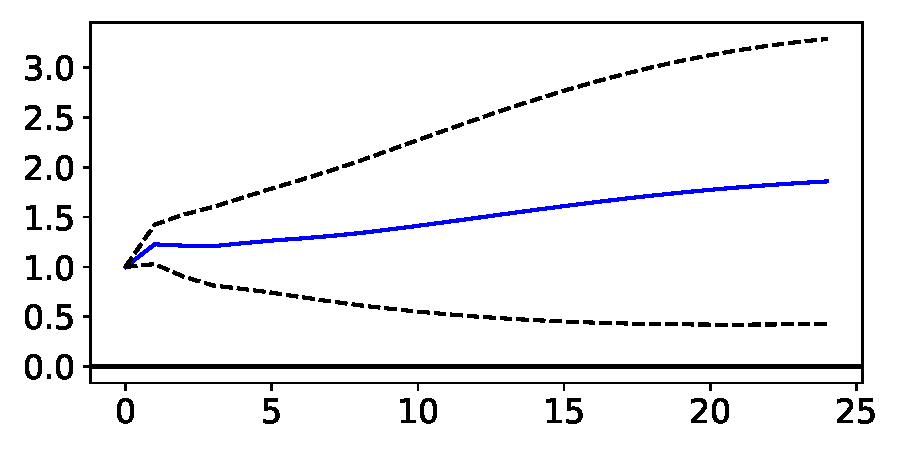
\includegraphics[width = \textwidth, scale=1]{irf/spread_spread.pdf}
            \caption{Impulso: spread}
        \end{subfigure}
        \begin{subfigure}[t]{.4\linewidth}
            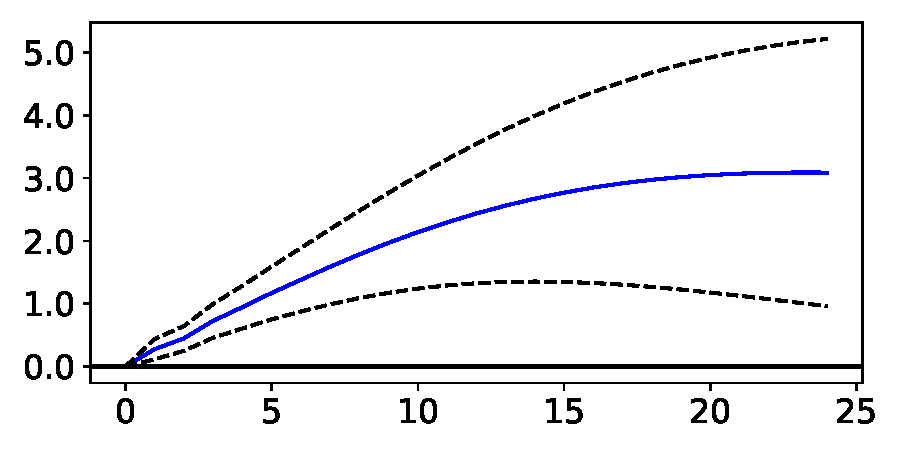
\includegraphics[width = \textwidth, scale=1]{irf/spread_selic.pdf}
            \caption{Impulso: selic}
        \end{subfigure}
        \begin{subfigure}[t]{.4\linewidth}
            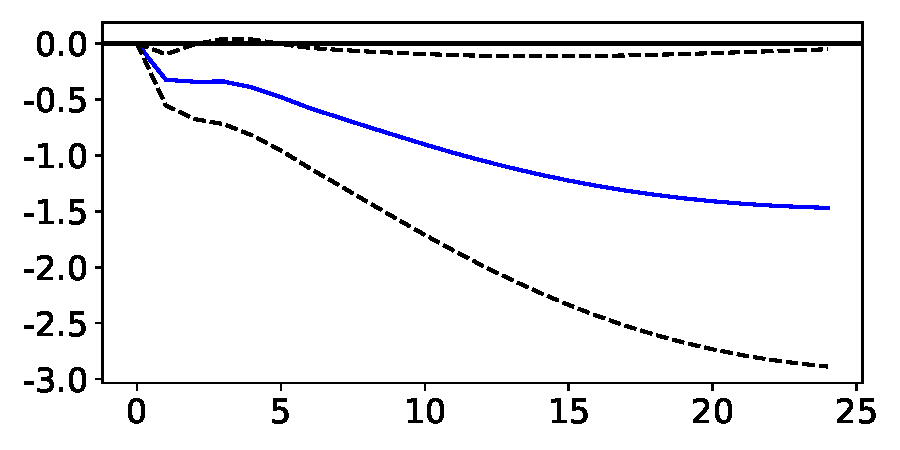
\includegraphics[width = \textwidth, scale=1]{irf/spread_inad.pdf}
            \caption{Impulso: inad}
        \end{subfigure}
        \begin{subfigure}[t]{.4\linewidth}
            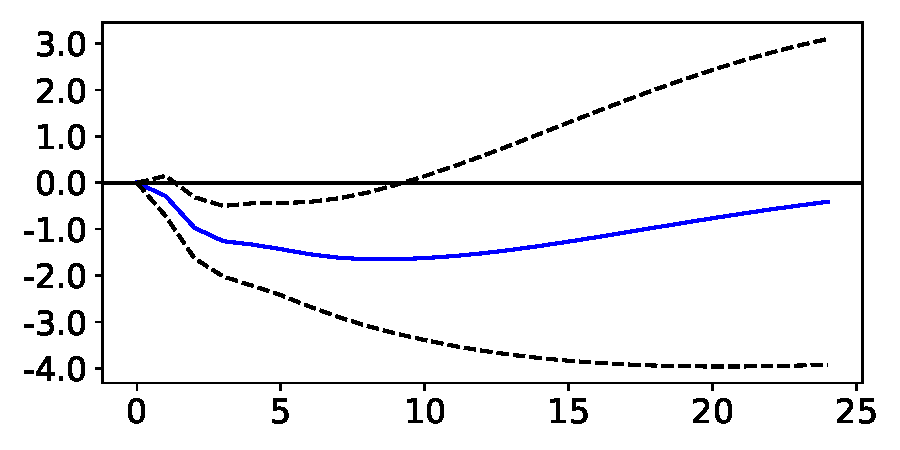
\includegraphics[width = \textwidth, scale=1]{irf/spread_ibc.pdf}
            \caption{Impulso: ibc}
        \end{subfigure}
    \end{figure}
\end{frame}


\begin{frame}
    \frametitle{Estimação do modelo vetorial de correção de erros}
    \framesubtitle{Funções de Impulso-resposta (ortogonal)}
    \begin{figure}[!hbt]
        \begin{subfigure}[t]{.4\linewidth}
            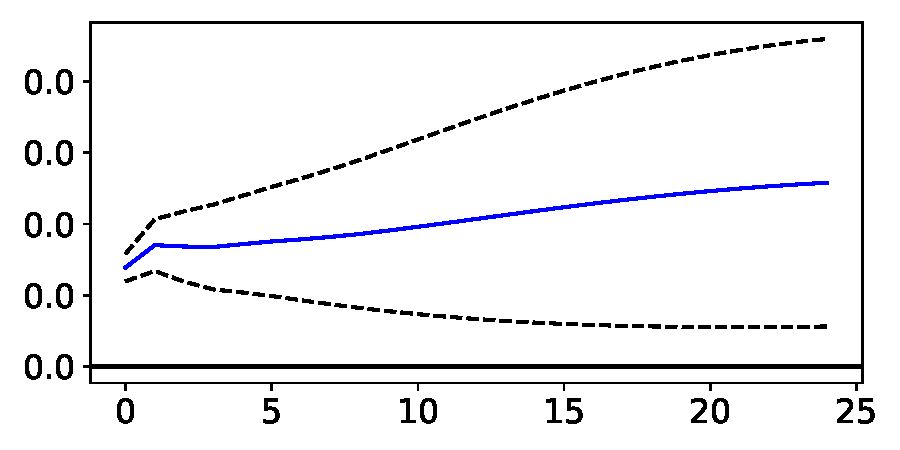
\includegraphics[width = \textwidth, scale=1]{irf/orth_spread_spread.pdf}
            \caption{Impulso: spread}
        \end{subfigure}
        \begin{subfigure}[t]{.4\linewidth}
            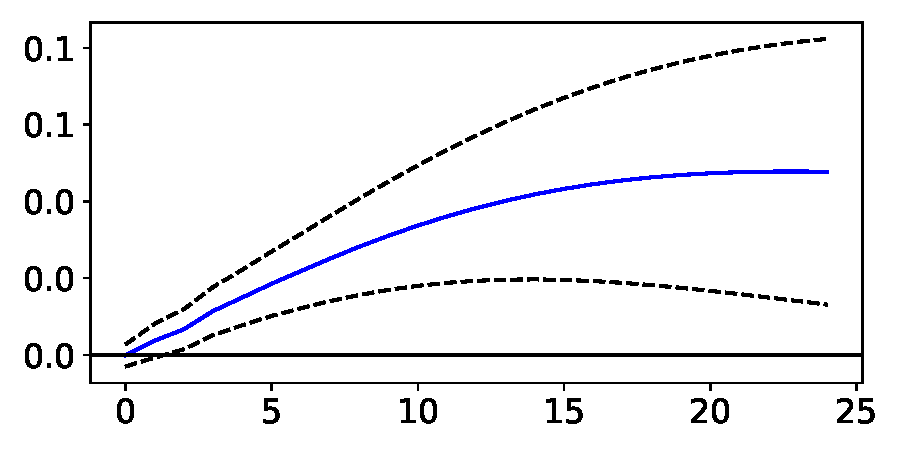
\includegraphics[width = \textwidth, scale=1]{irf/orth_spread_selic.pdf}
            \caption{Impulso: selic}
        \end{subfigure}
        \begin{subfigure}[t]{.4\linewidth}
            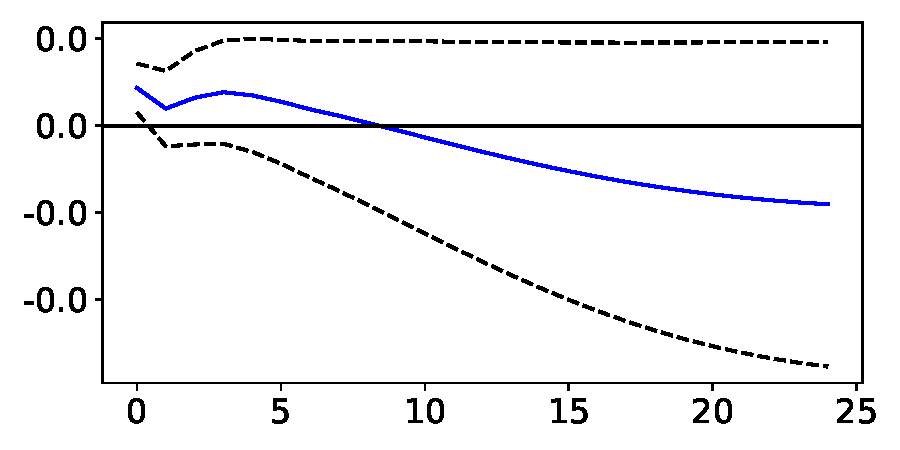
\includegraphics[width = \textwidth, scale=1]{irf/orth_spread_inad.pdf}
            \caption{Impulso: inad}
        \end{subfigure}
        \begin{subfigure}[t]{.4\linewidth}
            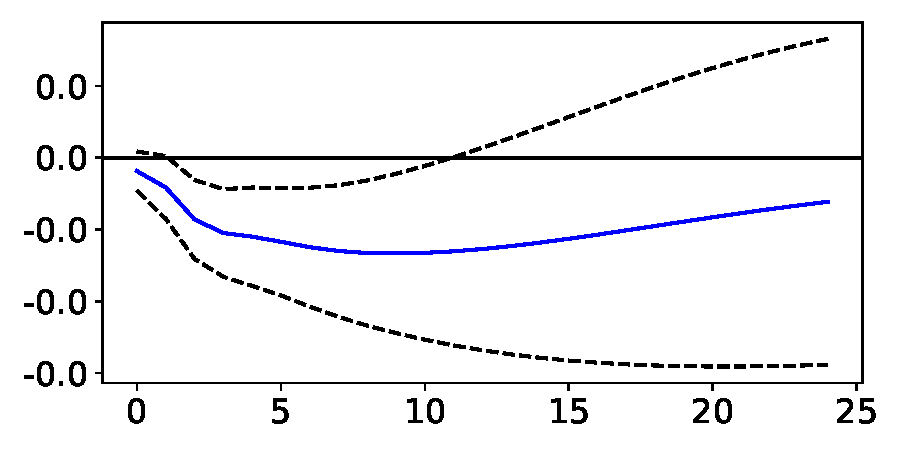
\includegraphics[width = \textwidth, scale=1]{irf/orth_spread_ibc.pdf}
            \caption{Impulso: ibc}
        \end{subfigure}
    \end{figure}
\end{frame}

\begin{frame}
    \frametitle{Conclusão}
    \begin{enumerate}
        \item A selic parece influenciar direta e persistentemente o nível do spread.
        \item A atividade econômica, no entanto, parece ser o que impede uma queda mais substancial.
        \item Os efeitos estimados da inadimplência vão contra o esperado. No entanto, seu efeito foi pouco significativo.
    \end{enumerate}
\end{frame}


\end{document}
